\chapter{UNIX システムとは何か}
\pagenumbering{arabic}

\ruby{UNIX}{ユニックス} システムとは、 \ruby{OS}{オーエス} の一種である。
そして、この本では、 \ruby{FreeBSD}{フリー・ビーエスディ} という
 OS を使って、 UNIX 系のシステムの使い方を紹介していく。
と言っても、よくわからないと思うので、まずこの章では OS、
それから UNIX システムなどについて簡単に説明することにしよう。

\section{OS とは何か}

短く説明すると、 OS とは、 \ruby{Operating System}{オペレーティング・システム}
(操作するためのシステム) の略で、コンピュータを快適に使いこなすための、
基本システムのプログラムである。

それでは、具体的に紹介していこう。

\subsection{どんな OS があるのか}

いわゆるパソコンと呼ばれているもので動く OS には、
 Microsoft 社の \ruby{Windows}{ウィンドウズ} シリーズ、
 Apple 社の \ruby{Mac OS}{マックオーエス} シリーズ、
東京大学の坂村教授の \ruby{TRON}{トロン}、
 \ruby{DOS}{ドス} と呼ばれるいくつかの OS、
そしてこの本で取り上げる UNIX 系のシステムなどがある。

パソコンで動く UNIX 系のシステムは、 PC-UNIX とも呼ばれていて、
 \ruby{Linux}{リナックス} や FreeBSD などがよく使われている。
また、 MacOS も \ruby{X}{テン}(version 10) 以降は、
 UNIX をベースとした OS になっている。

\begin{minipage}[H]{21zw}
\begin{figure}[H]
\centering{
\includegraphics[scale=1.0]{winxpdesktop.eps}}
\caption{Windows XP のデスクトップ}
\end{figure}
\end{minipage}
\hspace*{5mm}
\begin{minipage}[H]{21zw}
\begin{figure}[H]
\centering{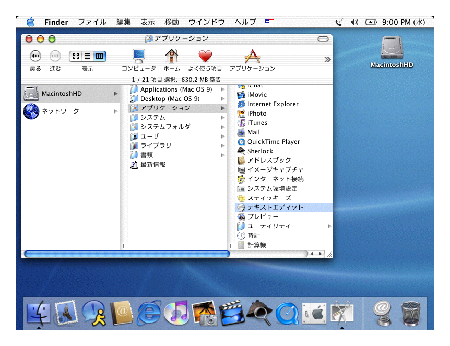
\includegraphics[scale=1.0]{MacOSXdesktop2.eps}}
\caption{Mac OS X のデスクトップ}
\end{figure}
\end{minipage}

\begin{minipage}[H]{21zw}
\begin{figure}[H]
\centering{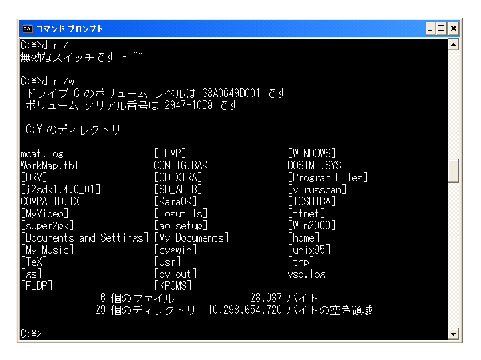
\includegraphics[scale=1.0]{MSDOSdesktop2.eps}}
\caption{MS-DOS コマンド・プロンプト}
\end{figure}
\end{minipage}
\hspace*{5mm}
\begin{minipage}[H]{21zw}
\begin{figure}[H]
\centering{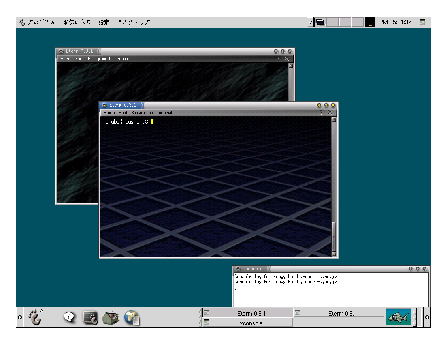
\includegraphics[scale=1.0]{gnomedesktop2.eps}}
\caption{FreeBSD のデスクトップ(GNOME使用)}\label{GNOME}
\end{figure}
\end{minipage}

\subsection{OS の役割とは}

コンピュータはいろいろなハードがつなぎ合わされて作られている。
これらをうまく適切にコントロールするには、
実際にはとても複雑な処理が必要となる。
その複雑な部分を包み込んで活用して、
ユーザから見たときには
簡単な操作でコントロールすることができるようにするのが OS の役割である。

%\bigskip

例えば、コンピュータでフロッピー・ディスクを使いたいとしよう。
 Windows の場合を思い出してみよう。
デスクトップにある「マイコンピュータ」というアイコンをクリックすると
ウィンドウが開いて、その中に「3.5 インチ FD」というアイコンが見える。
このアイコンがフロッピーを表してして、
更にクリックすると中に入っているファイルのリストを見ることができる。


\begin{figure}[H]
\centering{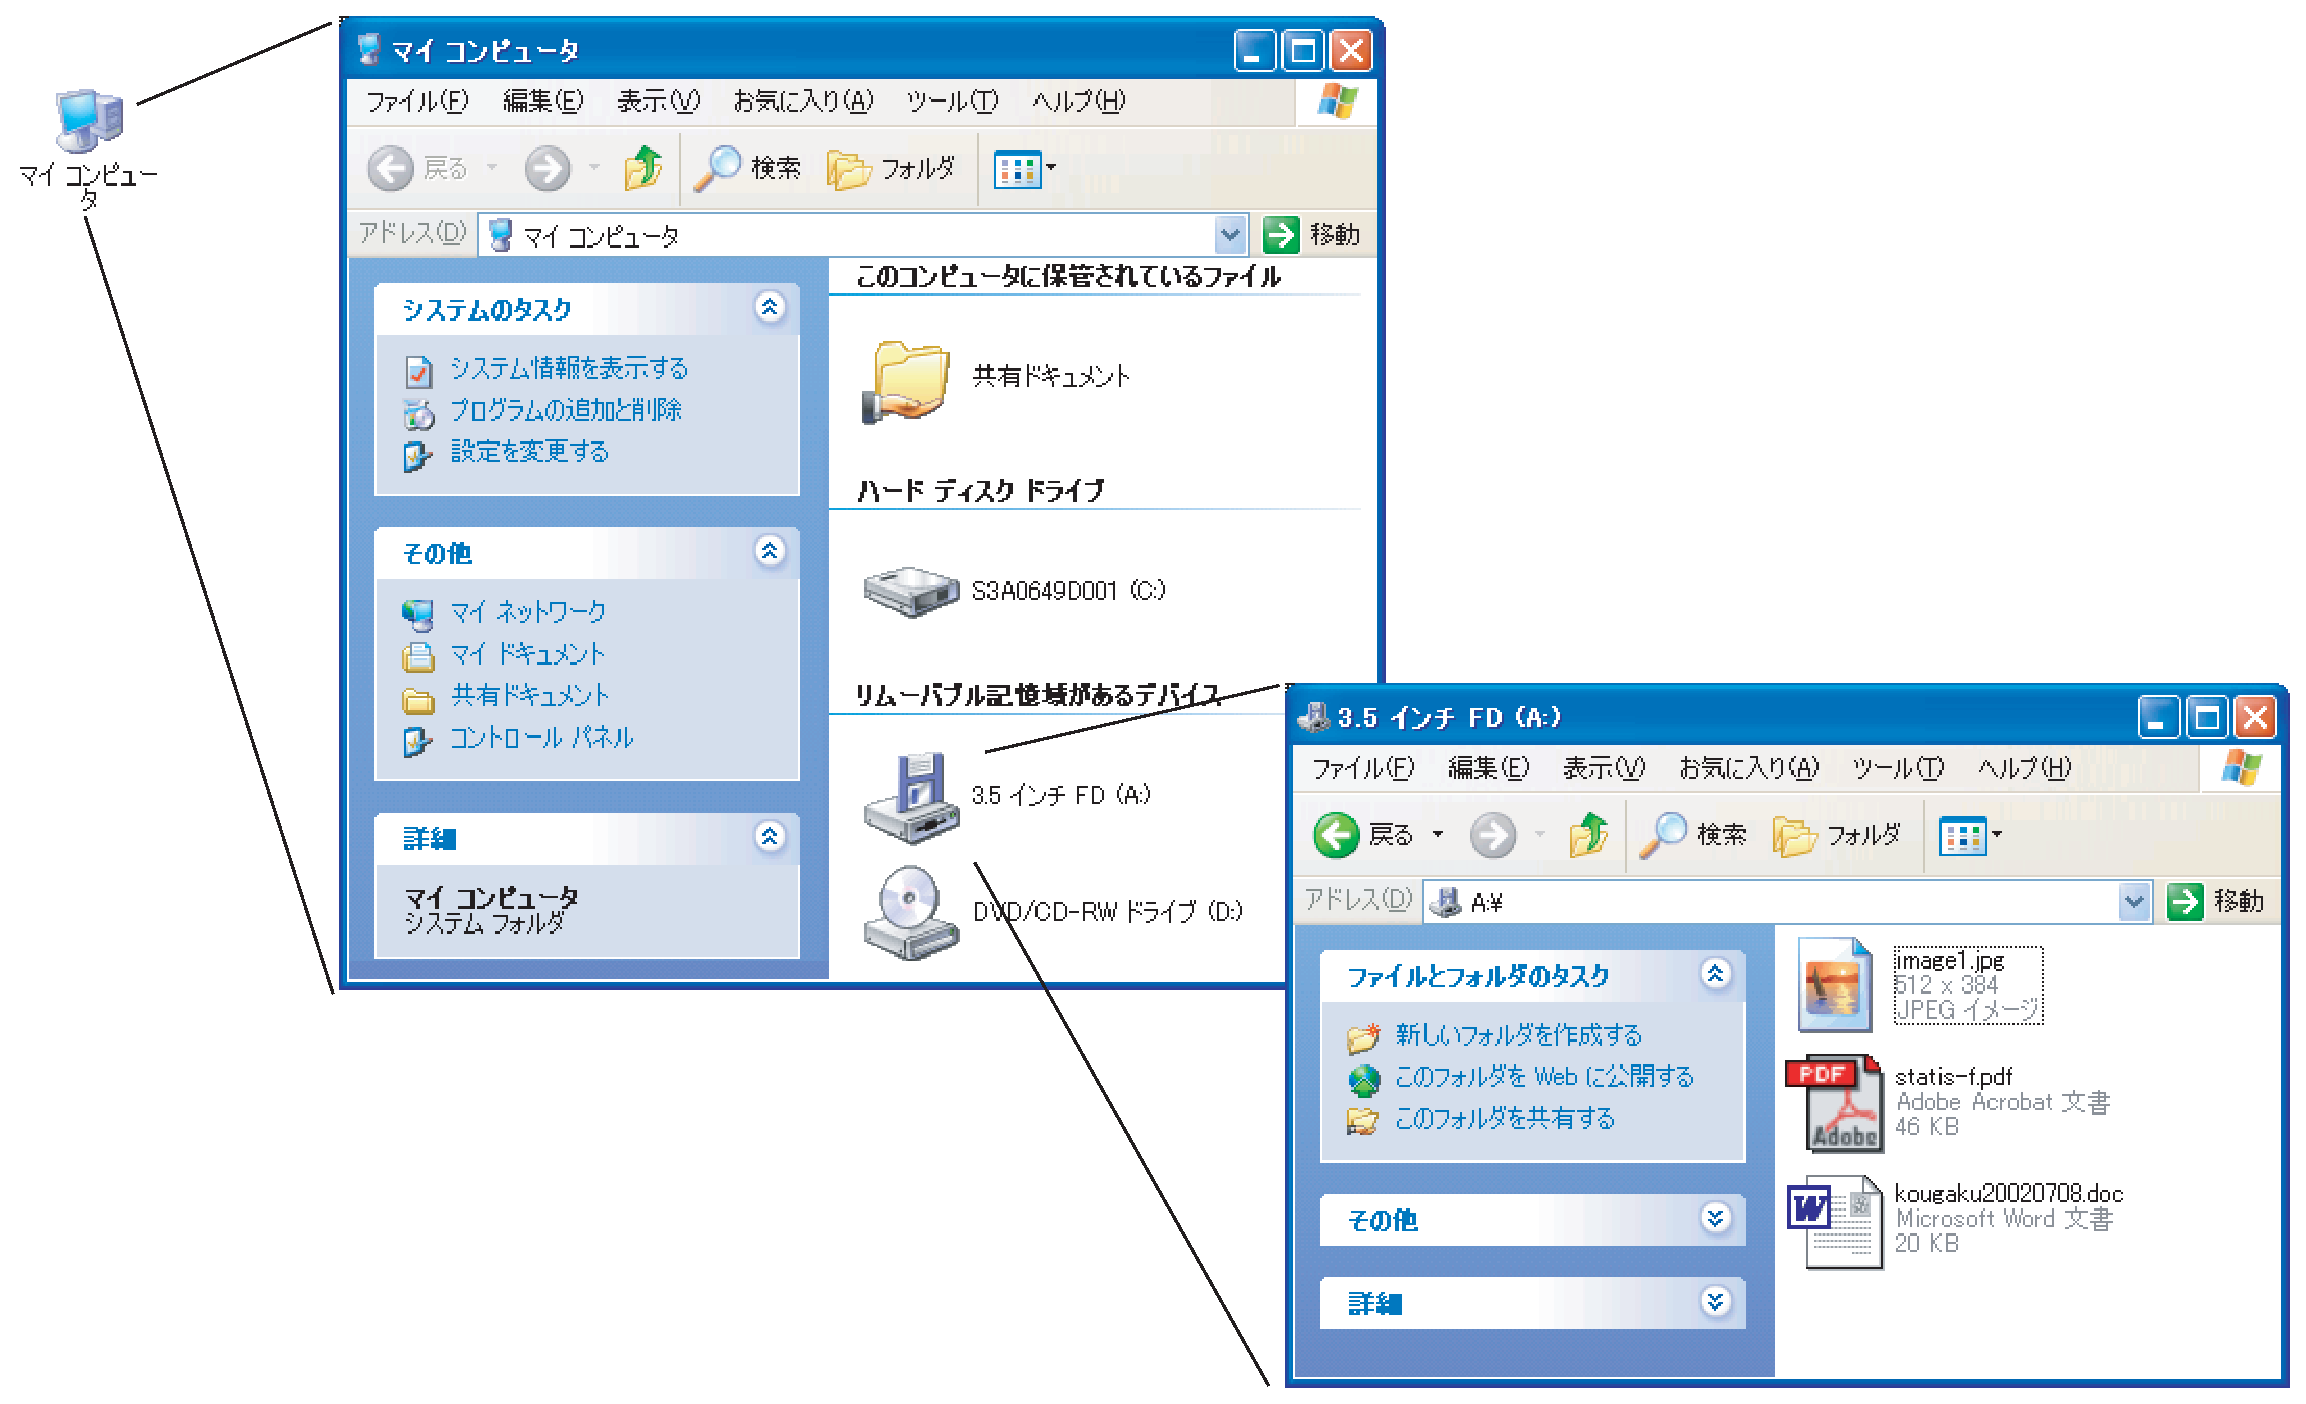
\includegraphics[scale=0.38]{winfloppy01.eps}}
\caption{Windows のファイル一覧}
\end{figure}

また、ファイルをフロッピー・ディスクにコピーするには、ファイルの
アイコンを持って、このフロッピーのアイコンに重ねてやればいい。

このようなアイコンの操作は、アイコンというシンボルを使って
簡略化、抽象化された「記号操作」の一種であると言える。

\begin{figure}[H]
\centering{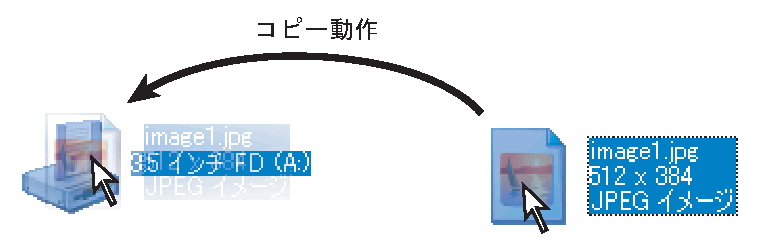
\includegraphics[scale=1.0]{wincopy01.eps}}
\caption{Windows でのファイルのコピー動作}
\end{figure}

ところで、このとき実際にコンピュータは何をしているのだろうか?

まず、フロッピーを回転させ、ドライブのヘッドをフロッピーに近づけて、
フロッピー上のどこにどんなデータが書かれているかというインデックスを
探して、それを読む。
次にファイルの中身を読むには、またヘッドを移動して・・・。

などという、気の遠くなるような複雑な操作が行なわれているのである。

\bigskip

こんなに複雑な操作を全部自分で一々やっていては、とてもコンピュータを
気軽には使えないだろう。

\begin{figure}[H]
\centering{
\includegraphics[scale=1.0]{readfloppy01.eps}}
\caption{フロッピーを読むときのハードウェアの動作}
\end{figure}

 Windows という OS では、このような複雑なハードに関する操作を
包み込んで見えないようにしている。
ユーザは単にアイコンをクリックするような「記号の操作」で、
簡単にコンピュータのシステムを使えるようになっているのである。
これは別に Windows だけでなく、他の OS でも同様である。

\newpage

\section{UNIX システムとはどういう OS か}

\subsection{UNIX システムの特徴}

 UNIX システムは 1970 年代のはじめに基本的な部分が開発され、
それ以降も発展し続けてきた歴史の長い OS である。
ちょっと難しい話になるが、最初に UNIX システムの特徴を短くまとめておこう。

\begin{enumerate}
\item \textbf{マルチユーザ}

一台のマシンを何人もの人が同時に使うことができる。
\item \textbf{マルチタスク}

一台のマシンで同時にいくつもの命令(タスク)を実行することができる。
\item \textbf{階層型ファイル・システム}

ファイル・システムがツリー状に構成されている。
\item \textbf{デバイスなどの取り扱いの統一}

周辺機器などのデバイスにいたるまですべてがファイルとして統一的に取り扱われる。
\item \textbf{ネットワーク機能}

システムが開発された初期の頃からネットワークを利用するためのシステムが用意されていた。
\item \textbf{主に C 言語で書かれたソース・コード}

システムの多くの部分が C 言語で書かれていて、
いろいろなマシンに移植しやすい。
\end{enumerate}

これらのいくつかの特徴は、現在では多くの OS に備えられ、
当たり前のこととなっているが、
当時としてはシンプルかつ先進的なものであった。

\subsection{UNIX システムと Windows}

具体的な話に入ろう。
 UNIX システムでは、 Windows とやり方は異なるものの、
文章を書いたり、プログラムを作ったり、電子メールやニュースを使ったり、
 WWW にアクセスしたり、絵を描いたりすることができる\footnote{ちなみに、
このテキストも、多くの部分は UNIX で作成している。}。

では、この 2 つの OS ではどこが違うのかを見てみよう。

\begin{enumerate}
\item \textbf{コマンド・ライン・ベースと GUI}

 UNIX では、基本的にコンピュータに何かをさせるときには、
コマンドをキーボードから打ち込む。
コマンドは簡単な英語を短縮したものが多い。
このようなシステムを、コマンド・ライン・ベースのシステムと呼ぶ。

一方、 Windows では、アイコンと呼ばれる「絵」をクリックしたり、
持って移動したりして、コンピュータを使う。
このようなシステムを \ruby{GUI}{ジーユーアイ}
(\ruby{Graphical}{グラフィカル} \ruby{User}{ユーザ} \ruby{Interface}{インタフェース})
のシステムと呼ぶ。

ただし、 UNIX 系のシステムでも、
\ruby{X}{エックス} \ruby{Window}{ウィンドウ} \ruby{System}{システム}
という GUI を使うことができ、 Windows のようにアイコンを用いて操作する
ことができる。
 X Window System はユーザの好みによって、大幅に環境を変えることが
できるという特徴を持っている。
特にウィンドウ・マネー

\begin{minipage}[H]{21zw}
\begin{figure}[H]
\centering{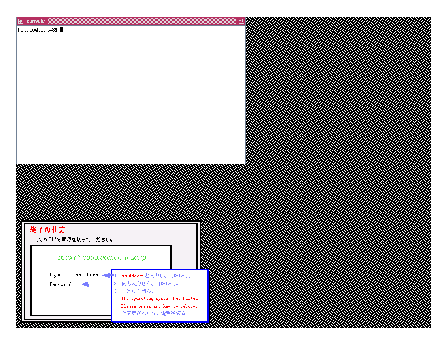
\includegraphics[scale=1.0]{twmdesktop2.eps}}
\caption{Twm}
\end{figure}
\end{minipage}
\hspace*{5mm}
\begin{minipage}[H]{21zw}
\begin{figure}[H]
\centering{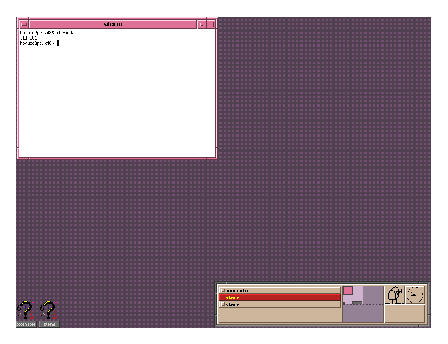
\includegraphics[scale=1.0]{fvwm2desktop2.eps}}
\caption{Fvwm}
\end{figure}
\end{minipage}

\begin{minipage}[H]{21zw}
\begin{figure}[H]
\centering{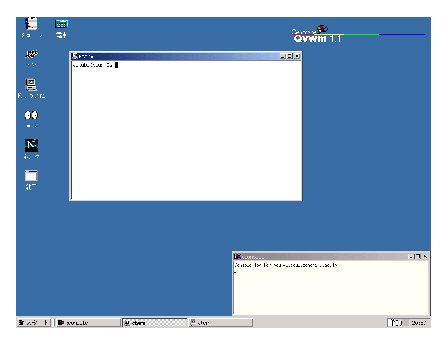
\includegraphics[scale=1.0]{qvwmdesktop2.eps}}
\caption{Qvwm}
\end{figure}
\end{minipage}
\hspace*{5mm}
\begin{minipage}[H]{21zw}
\begin{figure}[H]
\centering{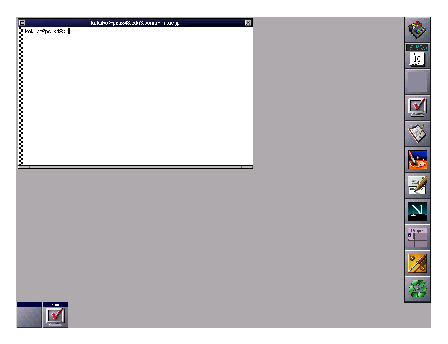
\includegraphics[scale=1.0]{afterstepdesktop2.eps}}
\caption{AfterStep}
\end{figure}
\end{minipage}

\begin{minipage}[H]{21zw}
\begin{figure}[H]
\centering{
\includegraphics[scale=1.0]{wmakerdesktop2.eps}}
\caption{WindowMaker}
\end{figure}
\end{minipage}
\hspace*{5mm}
\begin{minipage}[H]{21zw}
\begin{figure}[H]
\centering{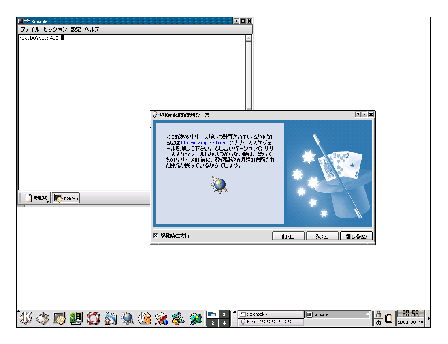
\includegraphics[scale=1.0]{kdedesktop2.eps}}
\caption{KDE}
\end{figure}
\end{minipage}

\begin{minipage}[H]{21zw}
\begin{figure}[H]
\centering{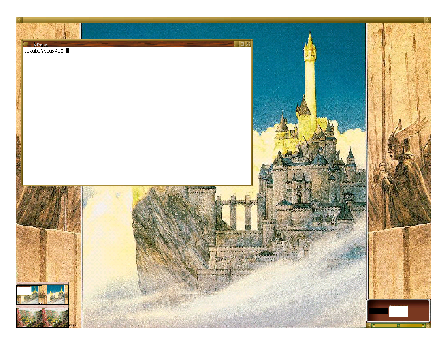
\includegraphics[scale=1.0]{enlightenmentdesktop2.eps}}
\caption{Enlightenment}
\end{figure}
\end{minipage}

\noindent
ジャーというソフトを変更すると、
全く異なった外見と操作方法になる。
ウィンドウ・マネー
ジャーには、図\ref{GNOME}の GNOME の他、
Twm、Fvwm、Qvwm、AfterStep、WindowMaker、KDE、Enlightenment などがある。

\item \textbf{マルチユーザとシングルユーザ}

UNIX 系のシステムでは、ネットワークごしにログインすることができて、
一台のマシンを同時に何人もで使うことができる。

例えば、何人もで同時にログインしてファイルを置いたりするようなことが
できる必要のある
インターネット・サービス・プロバイダの WWW サーバなどには、
 UNIX 系のシステムが使われていることが多い。

一方、 Windows は基本的にはコンピュータの前に座って、
一人で使うシステムである。
他のマシンからハードディスクの中身を見たりすることはできるが、
それ以上のことをするには特殊なソフトが必要になることが多い。

\item \textbf{オープンとクローズド}

UNIX 系のシステムのうち、特に Linux や FreeBSD は、
C 言語などで書かれたソース・コードは、完全にオープンになっている。

たとえば、 FreeBSD は \texttt{http://www.jp.freebsd.org/} が
日本の Web サイトである。
ここからすべて無料で自由にダウンロードすることができる。
ダウンロードしたソース・コードは中を読むこともできるし、
自分で自由にいじることもできる。

また、 Linux や FreeBSD の場合、 C コンパイラをはじめとした
数多くのプログラミング言語や便利なソフトウェアが無料で最初から付いていて、
わざわざお金をかけずに自由にプログラムを作ることができる。

一方、 Windows は商品であり、ソース・コードは一般に公開されていない。
 Windows 用のさまざまなソフトウェアも商品である場合が多い。
\end{enumerate}
